\documentclass[12 pt]{article}        	%sets the font to 12 pt and says this is an article (as opposed to book or other documents)
\usepackage{amsfonts, amssymb}					% packages to get the fonts, symbols used in most math
\usepackage{amsmath}
\usepackage{graphicx}\usepackage{multicol}
  
%\usepackage{setspace}               		% Together with \doublespacing below allows for doublespacing of the document

\oddsidemargin=-0.5cm                 	% These three commands create the margins required for class
\setlength{\textwidth}{6.5in}         	%
\addtolength{\voffset}{-2pt}        		%
\addtolength{\headsep}{25pt}           	%



\pagestyle{myheadings}                           	% tells LaTeX to allow you to enter information in the heading
\markright{Andrew Mayo\hfill \today \hfill}  
																									% and put the proposition number from the book
                                                	% LaTeX will put your name on the left, the date the paper 
                                                	% is generated in the middle 
                                                 	% and a page number on the right



\newcommand{\eqn}[0]{\begin{array}{rcl}}%begin an aligned equation - allows for aligning = or inequalities.  Always use with $$ $$
\newcommand{\eqnend}[0]{\end{array} }  	%end the aligned equation

%\doublespacing                         	% Together with the package setspace above allows for doublespacing of the document

\newcommand{\qed}[0]{$\square$}        	% make an unfilled square the default for ending a proof

\begin{document}												% end of preamble and beginning of text that will be printed 

\textbf{1 (c)} 

Test accuracy for CIFAR dataset: 42.08\%

\begin{figure}[h!]
  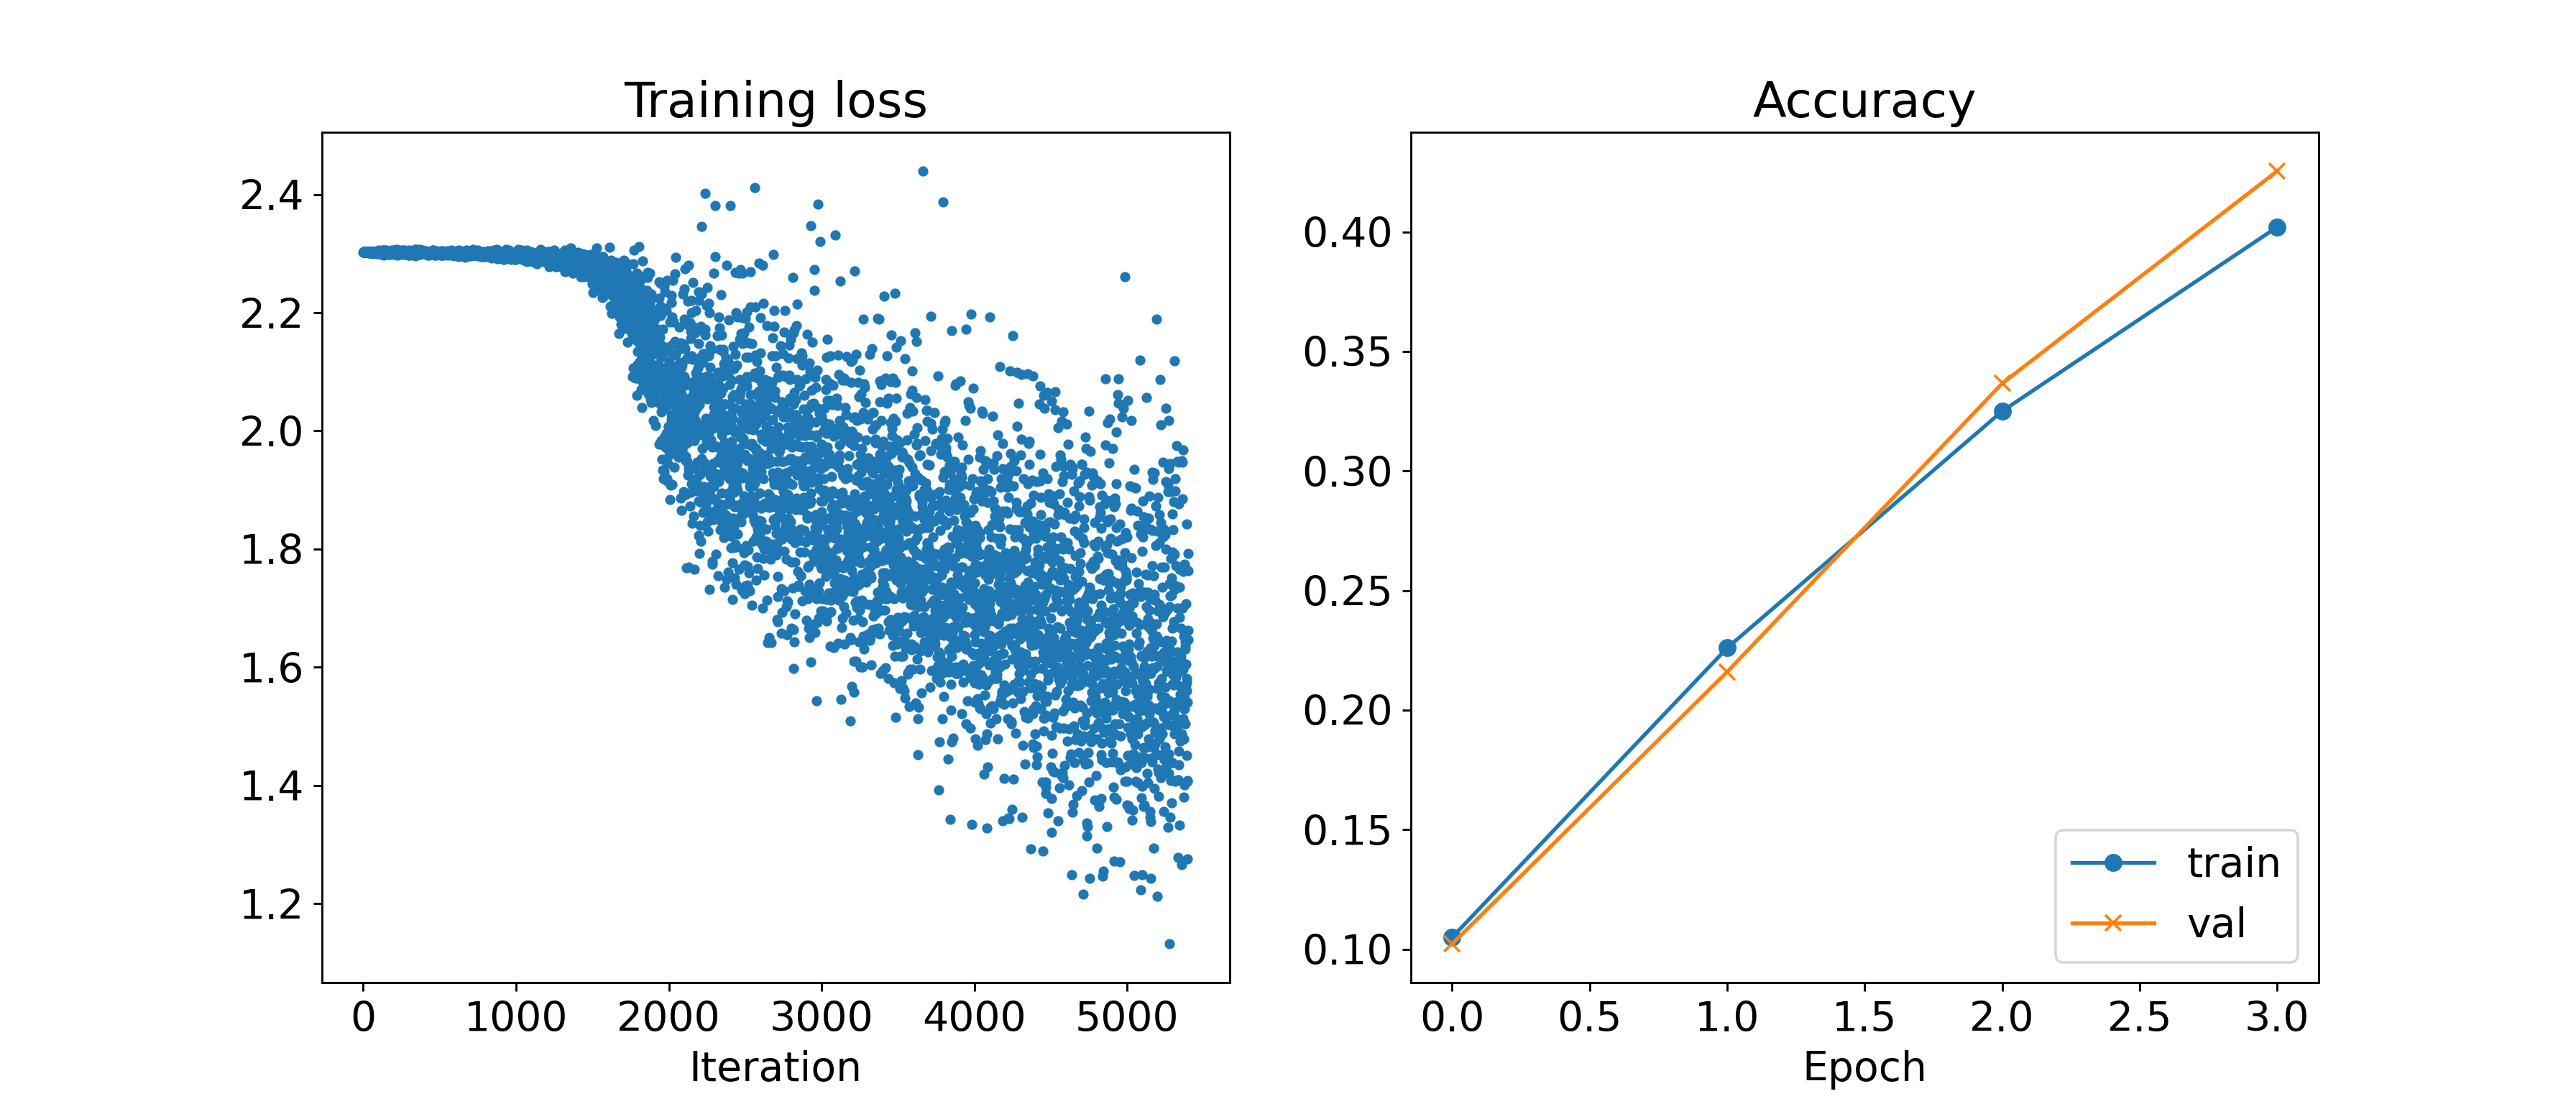
\includegraphics[width=\linewidth]{cnn.png}
\end{figure}


\textbf{2 (c)} 

\begin{figure}[h!]
  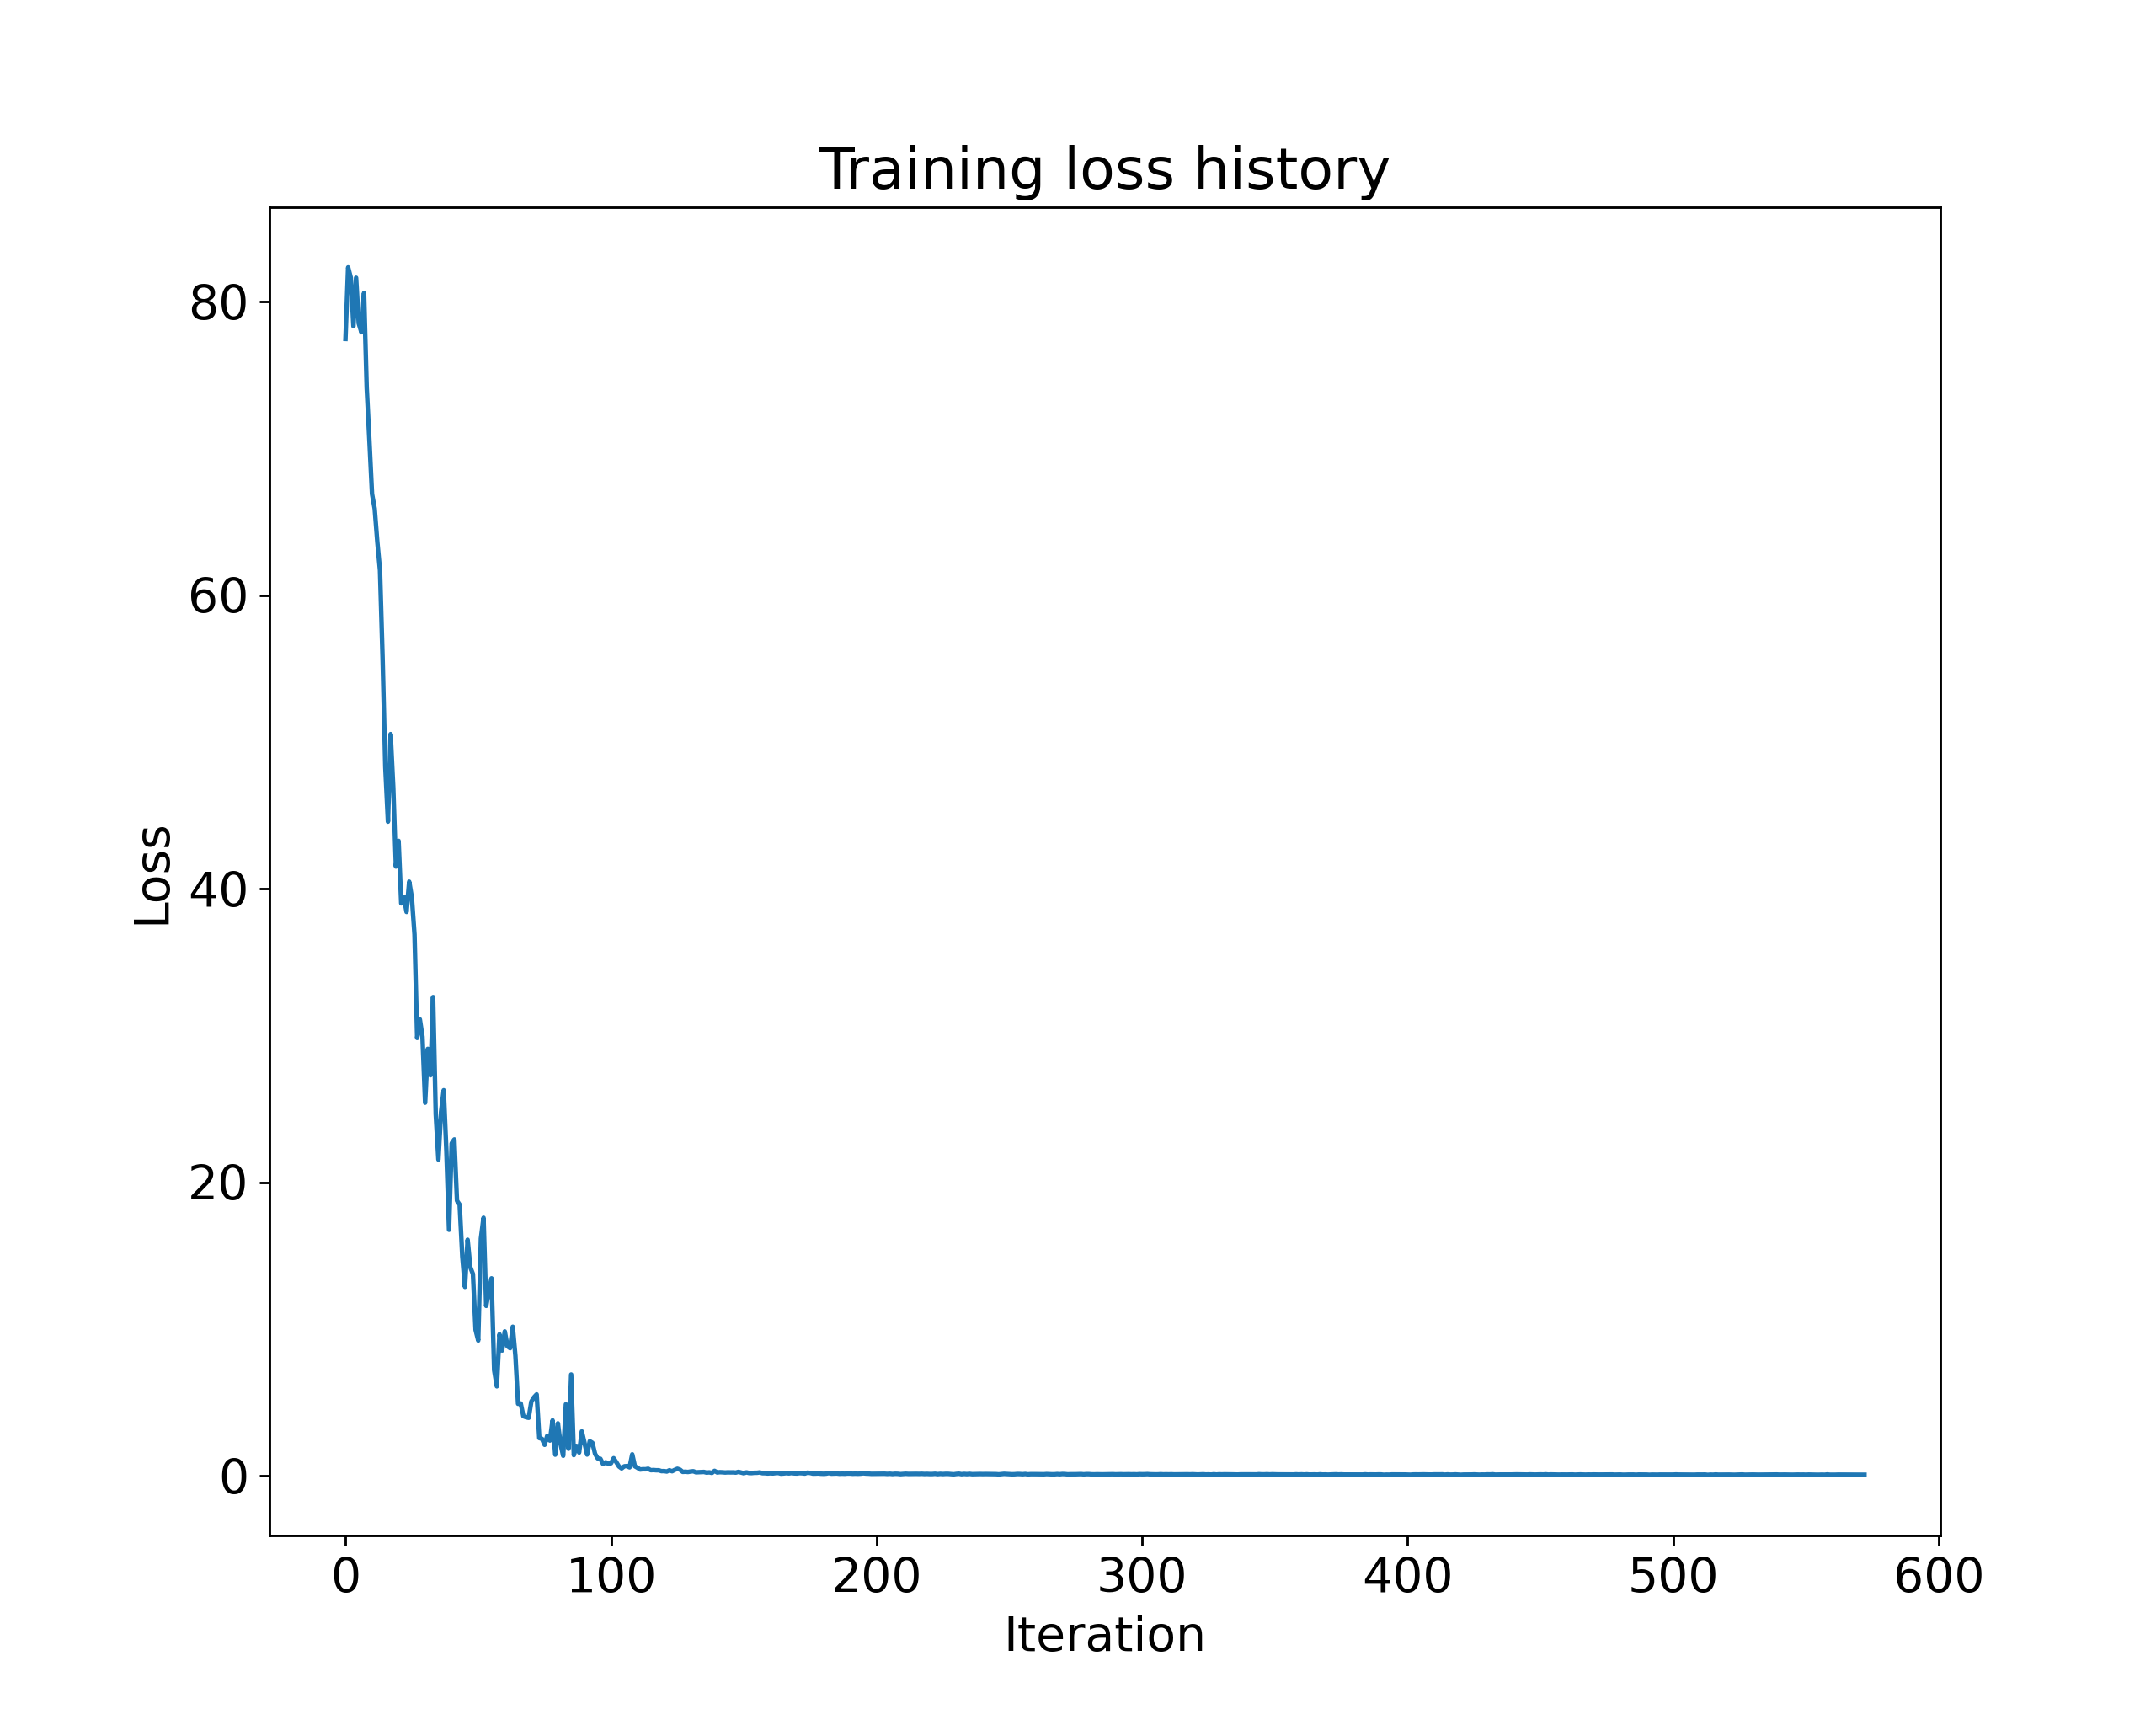
\includegraphics[width=0.5\linewidth]{image_captioning_loss.png}
\end{figure}

\begin{figure}[h!]
  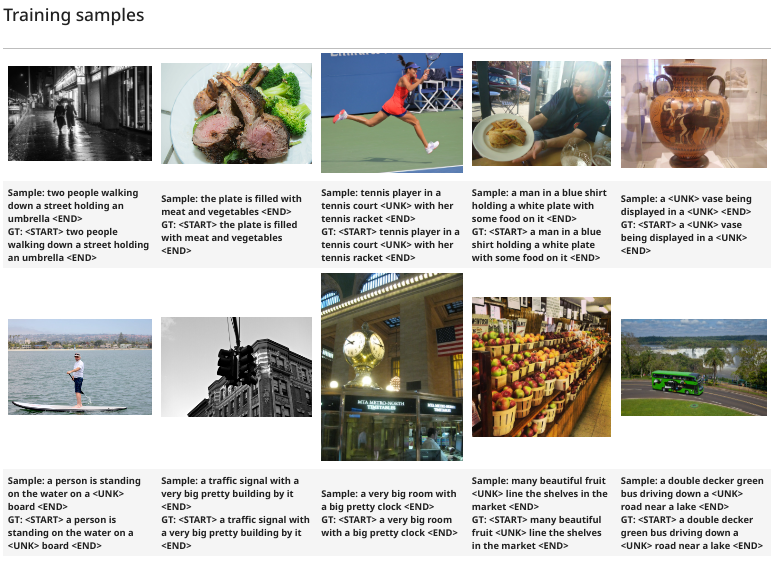
\includegraphics[width=0.7\linewidth]{captions_training.png}
\end{figure}

\begin{figure}[h!]
  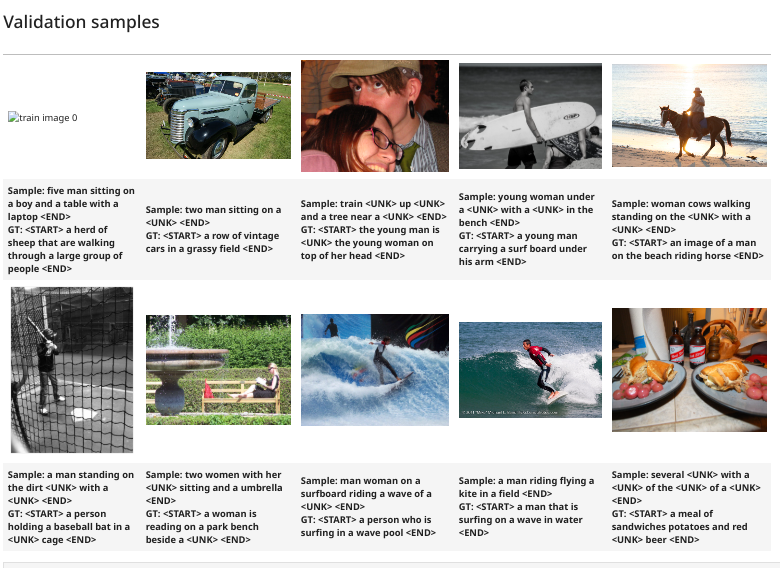
\includegraphics[width=0.7\linewidth]{captions_validation.png}
\end{figure}

\clearpage 

textbf{3 (b)}

\begin{multicols}{2}

\textbf{Fine-tuned pretrained model} \\

\begin{tabular}{ | c | c | } \hline
  Training time & 0m 0s \\
  Best val Acc & 0.712418 \\
  Epoch & 0/4 \\ \hline
        & \\
  train Loss & 0.5000 \\
  Acc & 0.7664 \\
  val Loss & 0.3085 \\
  Acc & 0.8758 \\
  Epoch & 1/4 \\ \hline
         & \\
  train Loss & 0.5936 \\
  Acc & 0.7254 \\
  val Loss & 0.2439 \\
  Acc & 0.9150 \\
  Epoch & 2/4 \\ \hline
        & \\
  train Loss & 0.5174 \\
  Acc & 0.7828 \\
  val Loss & 0.3162 \\
  Acc & 0.8824 \\
  Epoch & 3/4 \\ \hline
        & \\
  train Loss & 0.5208 \\
  Acc & 0.7705 \\
  val Loss & 0.3700 \\
  Acc & 0.8889 \\
  Epoch & 4/4 \\ \hline
        & \\
  train Loss & 0.7435 \\
  Acc & 0.7910 \\
  val Loss & 0.3417 \\
  Acc & 0.8562 \\
  Training time & 0m 6s \\
  Best val Acc & 0.915033 \\ \hline
\end{tabular}

\textbf{Without finetuning} \\

\begin{tabular}{ | c | c | } \hline
  Training time & 0m 0s \\
  Best val Acc & 0.457516 \\
  Epoch & 0/4 \\ \hline
        & \\
  train Loss & 0.5814 \\
  Acc & 0.7049 \\
  val Loss & 0.2089 \\
  Acc & 0.9346 \\
  Epoch & 1/4 \\ \hline
        & \\
  train Loss & 0.4798 \\
  Acc & 0.7910 \\
  val Loss & 0.1932 \\ 
  Acc & 0.9477 \\
  Epoch & 2/4 \\ \hline
        & \\
  train Loss & 0.5531 \\
  Acc & 0.7336 \\
  val Loss & 0.6048 \\
  Acc & 0.7647 \\
  Epoch & 3/4 \\ \hline
        & \\
  train Loss & 0.6411 \\
  Acc & 0.7418 \\
  val Loss & 0.1941 \\
  Acc & 0.9346 \\
  Epoch & 4/4 \\ \hline
        & \\
  train Loss & 0.4340 \\
  Acc & 0.8197 \\
  val Loss & 0.2179 \\
  Acc & 0.9281 \\
  Training time & 0m 4s \\
  Best val Acc & 0.947712 \\ \hline
\end{tabular}

\end{multicols}

\newpage

\textbf{3 (c)}

\begin{figure}[h!]
  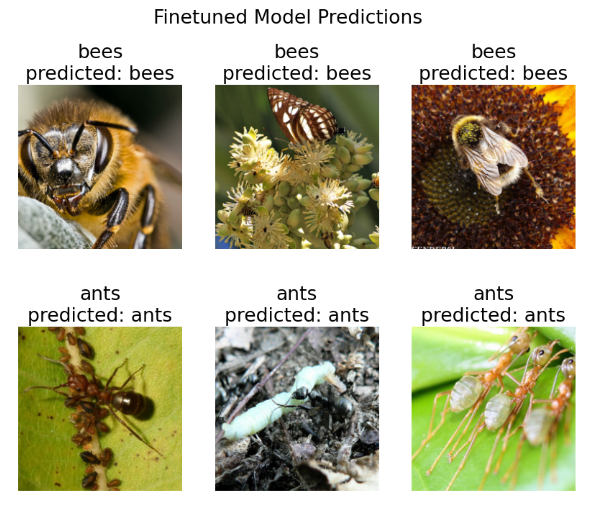
\includegraphics[width=0.6\linewidth]{tl_finetuned.png}
\end{figure}

\begin{figure}[h!]
  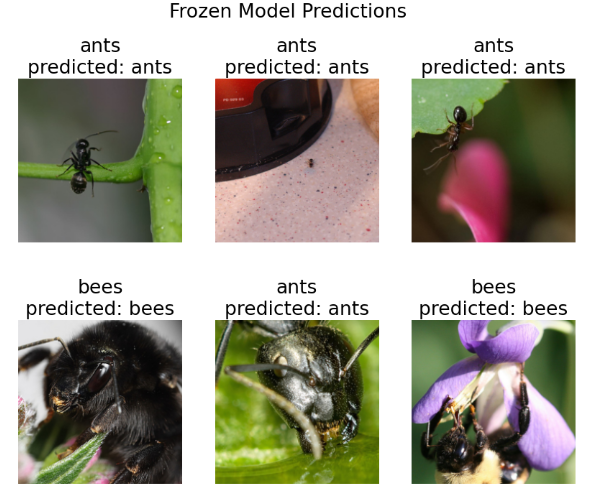
\includegraphics[width=0.6\linewidth]{tl_frozen.png}
\end{figure}


\end{document}
